\chapter{Blockchains as Cryptographic Data Structures}
Yet we have become familiar with blockchains, but now we discuss blockchains from another narrow point of view. We will look at blockchains as a data structure with cryptographic properties. We will see what properties this data structure satisfies and that's the key to a blockchain. Remember the two keywords for blockchains, decentralization, and trust. We should be able to link back these properties to trust, and perhaps decentralization.\\\\
We will discuss three basic cryptographic primitives :
\begin{enumerate}
    \item Cryptographic Hash Functions
    \item Hash Accumulators, Merkle trees
    \item Digital Signatures
\end{enumerate}
The first two primitives are combined to form a blockchain that enables trust, while the third primitive, signatures, allows for decentralization.\section{Hash Functions}
A hash function is a function that converts a binary string of arbitrary length to a binary string of fixed length. For any piece of data $x$, the output of the hash function is denoted by $H(x)$ and is called the hash of $x$. 
\ex{Division hashing}{\begin{align*}
        y = \, \, x \mod \,\, 2^{256}
    \end{align*} Think of $x$ as a binary sequence. This hash function modulates the input with $2^{256}$ and the output is a $256$-bit sequence, which is the remainder. Dividing by a large number of the remainder is uniform between $0$ and $2^{256} - 1$. It's a simple deterministic hash function that can be simply computed. \label{ex1.1.1}}

A \textbf{collision} happens when there are two inputs, $x$ and $x'$, which get mapped to the same hash, i.e., $H(x) = H(x')$.
To minimize collisions, a hash function must distribute its output uniformly and as spread-out as possible over the output space. Therefore, a good hash function should have the following properties:
\begin{enumerate}
    \item Arbitrary sized inputs
    \item Fixed-size deterministic output
    \item Efficiently computable
    \item Minimize collisions
\end{enumerate}
Hash functions are widely used not only in blockchains but also in databases, data mining, and information retrieval. They are beneficial for indexing lots of data, especially the ones that are not already numbers e.g. files, images and audio.
\section{Cryptographic Hash Function}
Cryptographic hash functions are quite the same as hash functions but with two extra properties:
\begin{enumerate}
    \item \textbf{adversarially collision resistance}
    \item \textbf{one way function}
\end{enumerate} 
The hash of a file should be unique and hard to replicate. An adversary should not be able to create another file that has the same hash as the original one. The previously provided example (\ref{ex1.1.1}) is not adversarially collision-resistant since we can simply add $2^{256}$ to the input and that will have the same output.\\
In this example, if we pick random inputs and compute the hash values, we’ll find a collision with high probability long before examining $2^{256} + 1$ inputs. In fact, if we randomly choose just $2^{130} + 1$ inputs, it turns out there’s a $99.8\%$ chance that at least two of them are going to collide. The fact that we can find a collision by only examining roughly the square root of the number of possible outcomes results from a phenomenon in probability known as the birthday
paradox .\\\\
The output space of cryptographic hash functions must be large. Otherwise, one could easily find a hash collision by iterating over the output space. Typically, they are 128-bit strings, 256-bit strings, or longer.\\\\
The key feature of a cryptographic hash function is that it is easy to compute but difficult to invert. This means that given a binary string $x$, it is easy to compute $y = H(x)$, but given an arbitrary $y'$, it is difficult and it would take a really long time to find any $x'$ for which $H(x') = y'$.
\subsection*    {SHA-256}
Constructing a cryptographic hash function is not easy (in contrast to regular hash functions). The National Institute of Standards and Technology (NIST) sets a standard for these hash functions. One such function is \textbf{SHA-256}, where SHA stands for Secure Hash Algorithm, and 256 is the length of the output. \\
They are built using the Merkle–Damgård construction, from a one-way compression function.\\\\
A hash of a certain value acts as a commitment to that value. One can broadcast the hash of the value instead of the value itself. Due to the collision-resistance property, one cannot generate an alternate value that matches the same hash
value; one is committed to the original value. Thus, publishing the hash of a value is like writing it on a piece of paper and placing it in a sealed envelope.
\section{Hash Pointer and chains of block}
A hash function can also be used as a pointer to certain values when these are stored in a hash table. Note that a hash pointer is nothing more than a hash; the term alludes to the fact that the hash is being used as a pointer.\\
Hash pointer retrieves information and verifies that the information has not changed. Hash pointers can also be used to build related data structures which is crucially useful for blockchains. In fact, the blockchain itself is a hash pointer-based data structure. \\\\
In the context of blockchains, a block is a data type that contains a particular header field, called the \textbf{hash pointer}, and some \textbf{data}.\\
Using the hash pointer, we build a linked list (See figure \ref{fig:f1}). We’re going to call this data structure a blockchain. Whereas in a regular linked list where you have a series of blocks, each block has data as well as a pointer to the previous block in the list, in a blockchain the previous block pointer will be replaced with a hash pointer. Thus, each block not only tells us where the value of the previous block was, but also contains a digest of that value that allows us to verify that the value hasn’t changed. We store the head of the list, which is just a regular hash pointer that points to the most recent data block.
\begin{center}
	\begin{figure}
		\centering
		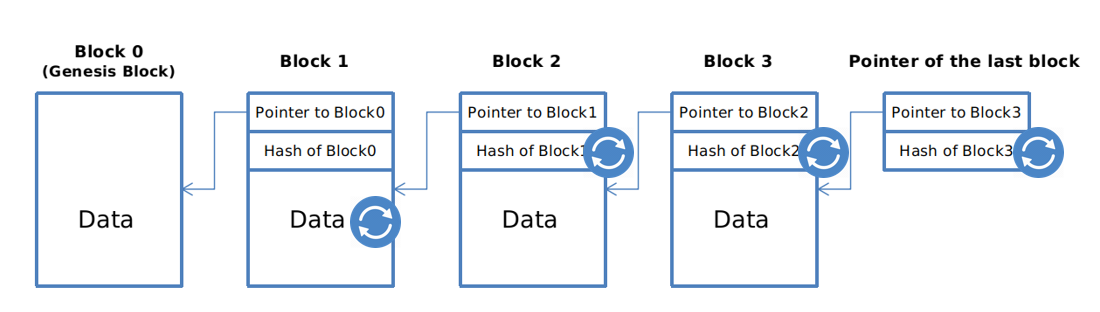
\includegraphics[width=0.8\linewidth]{Fig/02/F1}
		\caption{A block chain is a linked list that is built with hash pointers instead of pointers}
		\label{fig:f1}
	\end{figure}
\end{center}
A use case for a blockchain is a tamper‐evident log. That is, we want to build a log data structure that stores a bunch of data and allows us to append data to the end of the log. But if somebody alters the data that is earlier in the log, we’re going to detect it.\\\\
Blockchains are tamper-proof data structures, making them particularly useful in digital trust systems. The system consists of parties that keep their own hash tables as local copies of the data structure. A party can trace the lineage of any block (its parent, grandparent, etc.) using the hash pointers. If a party is missing a block in its hash table, it can ask its peers for the block by using the hash of the block (which it gets from the child block). It can then confirm that the block it gets from its peer is the right one (i.e., it has not been altered) by checking if its hash matches with what it has; this is essentially using the hash as a proof. Likewise, a party can verify if any part of the blockchain it receives has been changed or not.\\
A party may want to check if a specific data value is part of the blockchain. If the party has the whole blockchain and all its internal data, it can easily prove this. But for a party that only cares about one data value, this is too much work. To make this easier for practical blockchain systems, we use a Merkle tree data structure to store the data in each block. We will explain this next.
\section{Merkle tree}
Another useful data structure that we can build using hash pointers is a binary tree. A binary tree with hash pointers is known as a Merkle tree, after its inventor Ralph Merkle.
\begin{figure}[h!]
	\centering
	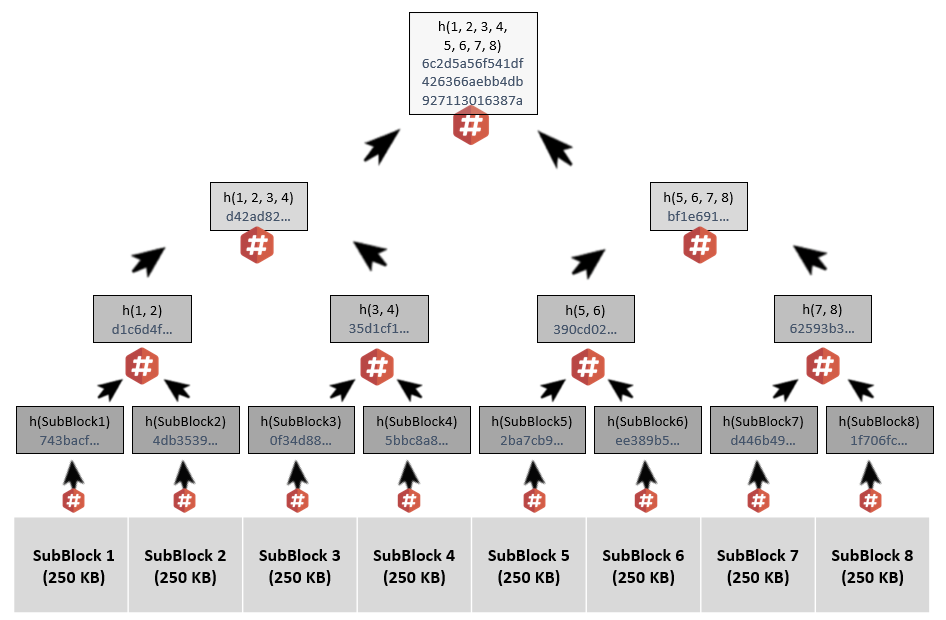
\includegraphics[width=0.65\linewidth]{Fig/02/F2}
	\caption{A Merkle tree}
	\label{fig:f2}
\end{figure}
Suppose we have a number of blocks containing data. We group these data blocks into pairs of two, and then for each pair, we build a data structure that has two hash pointers, one to each of these blocks. We continue doing this until we reach a single block, the root of the tree.

\begin{figure}[h!]
    \centering
    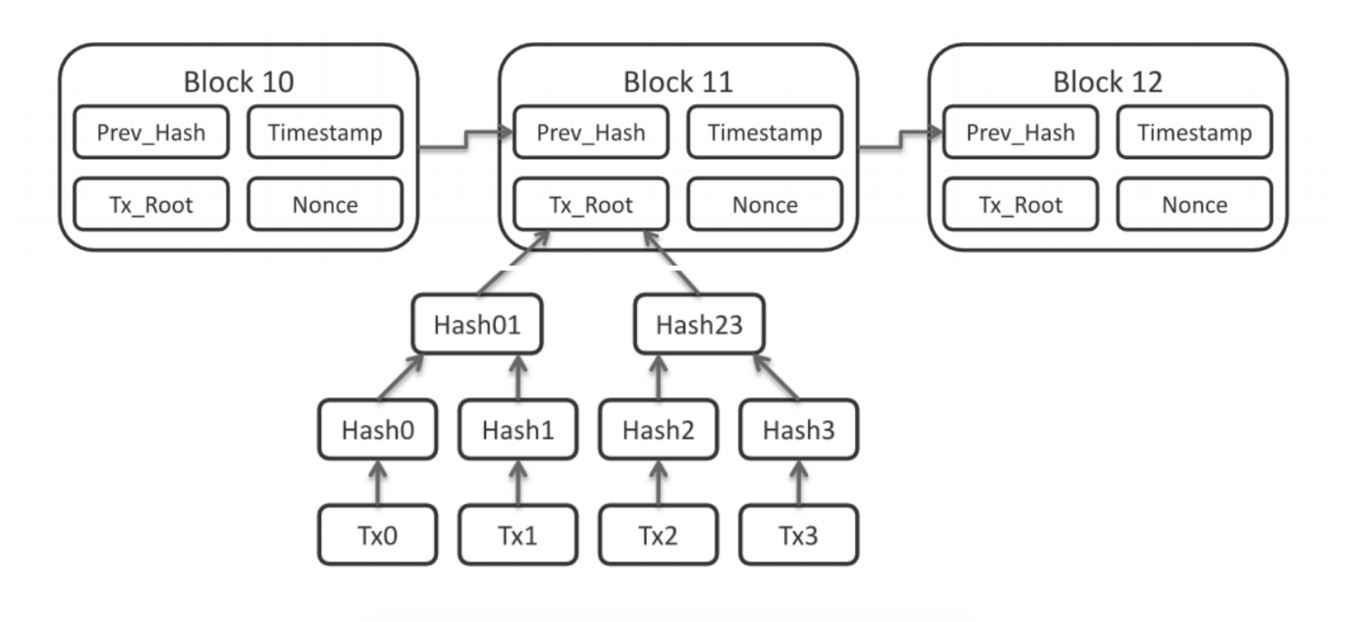
\includegraphics[width=0.65\linewidth]{Fig/02/F4}
    \caption{Blockchain with Markle trees}
    \label{fig:f4}
\end{figure}

As you see above, we have a blockchain and the data of each block is stored as a markle tree. We don't just keep the hash of data, we always keep the hash of markle. In this case header contains the hash of the previous block and the root of markle tree.

\subsection*{Proof of membership}
Say that someone wants to prove that a certain data block is a member of the Merkle Tree. As usual, we remember just the root. Then they need to show us this data block, and the blocks on the path from the data block to the root. We can ignore the rest of the tree, as the blocks on this path are enough to allow us to verify the hashes all the way up to the root of the tree.
\begin{center}
    \begin{figure}[h!]
        \centering
        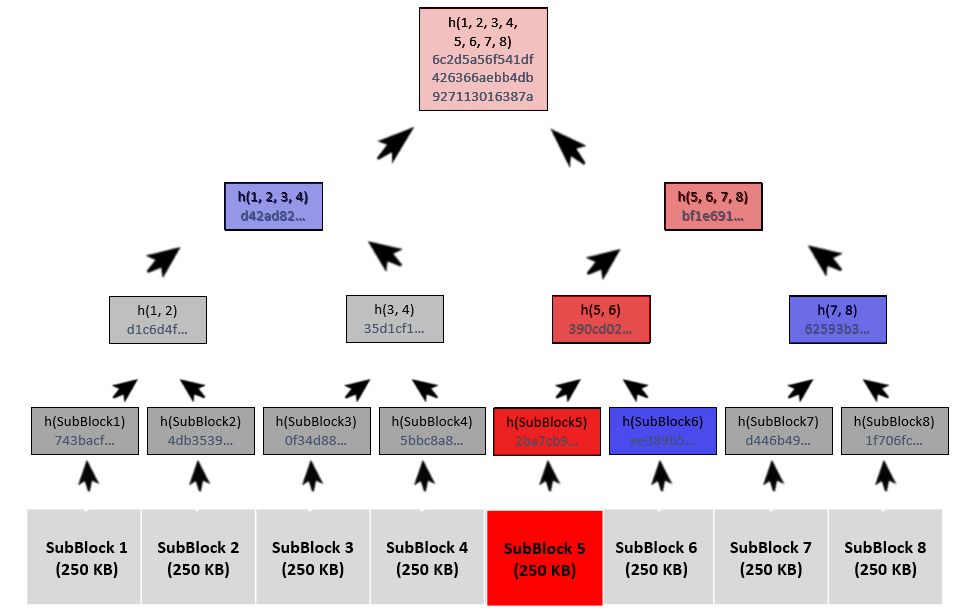
\includegraphics[width=0.7\linewidth]{Fig/02/F3}
        \caption{Finding a block in Merkle tree}
        \label{fig:f3}
    \end{figure}
\end{center}
If there are n nodes in the tree, only about log(n) items need to be shown. And since each step just requires computing the hash of the child block, it takes about log(n) time for us to verify it.
\subsection*{Proof of non‐membership}.
With a sorted Merkle tree, it becomes possible to verify non‐membership in a logarithmic time and space. That is, we can prove that a particular block is not in the Merkle tree. The way we do that is simply by showing a path to the item that’s just before where the item in question would be and showing the path to the item that is just after where it would be. If these two items are consecutive in the tree, then this serves as proof that the item in question is not included. If it was included, it would need to be between the two items shown, but there is no space between them as they are consecutive.
\section{Digital Signature}
Digital signatures serve as the cryptographic equivalent of handwritten signatures. They enable anyone to verify the sender of a message. In a digital signature scheme, each user is provided with a pair of keys: a secret key known only to the user and a public key shared with everyone.
To sign a message, a user employs their secret key, and the resulting signature is sent alongside the message. Another user can verify that the message indeed came from the purported sender by comparing the message and signature to the sender's public key. Thus, the public key becomes the user's identity in the system.

The security of a digital signature scheme lies in the inability of an adversary to forge signatures without knowledge of the corresponding secret key.

It is crucial that each message has a distinct signature. If the same signature could be used for multiple messages, an adversary could simply append the signature to other messages, rendering the scheme ineffective. Typically, users sign the hash of the message they intend to send, ensuring a constant-length bit string for both the signed object and the signature.

To ensure unforgeability, the signature length must be sufficient. Secure signature schemes are standardized by organizations such as NIST.

Bitcoin utilizes the Elliptic Curve Digital Signature Algorithm (ECDSA) as its signature scheme. Elliptic curves are employed in the signing process, but the details are beyond the scope of this discussion. Further information on ECDSA can be found on the Wikipedia page and associated links.

Digital signatures find their first application in upgrading a centralized blockchain system to a decentralized version. Each block in the blockchain is augmented with a digital signature, enabling different users to append blocks and identify themselves through their signatures.

In this decentralized architecture, there are three key questions to address:
\begin{enumerate}
	\item { Who are the eligible users allowed to participate, and how are they selected?}
	\item {When and which block can a user append, and how can others verify this rule in a decentralized manner?}
	\item {Where should a user append a block? In theory, a block can be attached to any other block as viewed by the user.}
\end{enumerate} 


Blockchain designs vary in how they answer these three questions and the properties they possess. In the next lecture, we will explore how Bitcoin resolves these questions.

The second application of digital signatures involves providing user attribution to the data stored in blocks. While the data is considered an abstract digital entity, there are scenarios where attributing it to users is essential. For example, in cryptocurrencies, the data represents transactions that record the transfer of ownership of coins. By using signatures, user ownership of coins can be established during the creation stage and subsequent ownership transfers can be verified.

\section{Summary}
Hash functions map any value or data to a fixed-size bit string. The hash of a value is typically unique and serves as its identifier. Hash functions play a vital role in constructing tamper-proof data structures like blockchains and Merkle trees.

Hashes provide commitments to data, ensuring its integrity and authenticity. Additionally, Merkle trees serve as accumulators and enable proof of membership for individual elements within a committed set.

Digital signatures function similarly to handwritten signatures, providing authentication in communication. In a blockchain system, all exchanged messages are signed to ensure their authenticity.

We previously introduced ledgers as ordered lists of data values. The blockchain and Merkle tree structures are sufficient to create a centralized ledger, with a central authority responsible for writing to the ledger and multiple parties reading from it.

Digital signatures play a crucial role in transitioning from a centralized ledger to a decentralized one.

To achieve a functional decentralized ledger, three important questions need to be addressed:
\begin{enumerate}
    \item {Who can participate in the ledger, and how are participants chosen?}
    \item {How can users append blocks to the ledger, and how can this process be verified in a decentralized manner?}
    \item {Where should a user append their block? In a decentralized ledger, blocks can be attached to any existing block as perceived by the user.}
\end{enumerate} 
